% Defining the LaTeX document class
\documentclass[a4paper,12pt]{article}

% Including necessary LaTeX packages
\usepackage{amsmath}
\usepackage{graphicx}
\usepackage{tikz}
\usepackage{geometry}
\geometry{margin=1in}
\usepackage{listings}
\usepackage{xcolor}
\usepackage{caption}
\usepackage{float}          % For [H] placement
\usepackage{noto}           % Font package, loaded last

% TikZ libraries for better rendering
\usetikzlibrary{arrows, positioning}

% Setting up code listing style
\lstset{
    basicstyle=\ttfamily\small,
    breaklines=true,
    frame=single,
    numbers=left,
    numberstyle=\tiny,
    keywordstyle=\color{blue},
    stringstyle=\color{red},
    commentstyle=\color{green!50!black}
}

% Starting the document
\begin{document}

% Creating the title
\title{Introduction to Forward Propagation in Neural Networks}
\author{}
\date{}
\maketitle

% Abstract section
\begin{abstract}
This report introduces forward propagation in neural networks, featuring a custom-designed neural network with three input neurons, two hidden layers (with three and two neurons, respectively), a third hidden layer with two neurons, and a final output layer with one neuron. The hidden layers use ReLU activation, except for the third hidden layer, which uses sigmoid activation, and the final output layer also uses sigmoid activation. The network is implemented using a custom approach with hand calculations, followed by implementations in Python, TensorFlow, and PyTorch. Weights, biases, and inputs are integers between 1 and 20, with the input as a column vector and weight matrices transposed during calculation. A diagram of the neural network architecture is included, along with a placeholder for a screenshot of the output for verification.
\end{abstract}

% Section for Neural Network Design
\section{Neural Network Design}
The neural network consists of:
\begin{itemize}
    \item \textbf{Input Layer}: 3 neurons
    \item \textbf{Hidden Layer 1}: 3 neurons (ReLU activation)
    \item \textbf{Hidden Layer 2}: 2 neurons (ReLU activation)
    \item \textbf{Hidden Layer 3}: 2 neurons (Sigmoid activation)
    \item \textbf{Final Output Layer}: 1 neuron (Sigmoid activation)
\end{itemize}
Weights, biases, and inputs are initialized as integers between 1 and 20, with the input vector as a column vector, and weight matrices transposed during each calculation step.

% Subsection for Network Diagram
\subsection{Network Diagram}
\begin{figure}[H]  % Fixed position using [H]
    \centering
    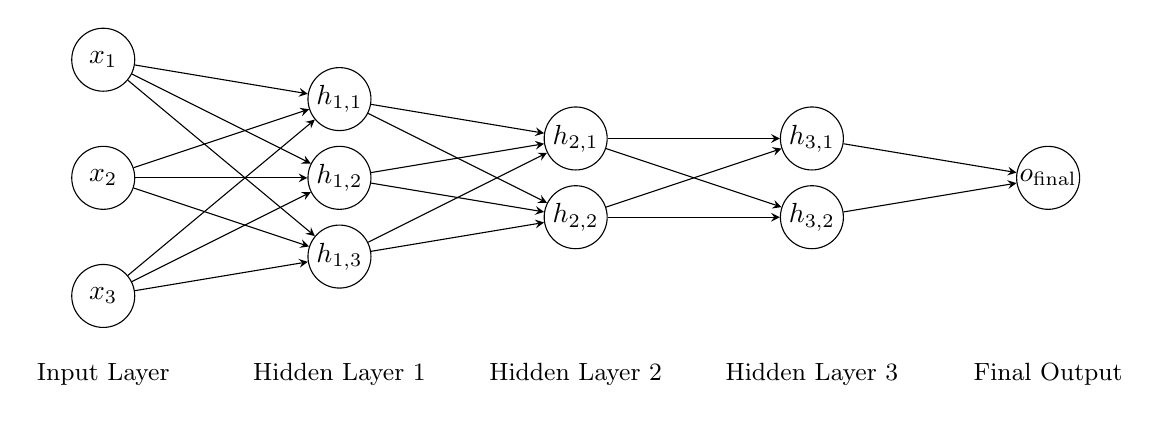
\begin{tikzpicture}[
        neuron/.style={circle, draw, minimum size=0.8cm, inner sep=0pt},
        layer/.style={font=\small},
        >=stealth
    ]
        % Input Layer
        \node[neuron] (I1) at (0,0) {$x_1$};
        \node[neuron] (I2) at (0,-1.5) {$x_2$};
        \node[neuron] (I3) at (0,-3) {$x_3$};
        
        % Hidden Layer 1
        \node[neuron] (H1_1) at (3,-0.5) {$h_{1,1}$};
        \node[neuron] (H1_2) at (3,-1.5) {$h_{1,2}$};
        \node[neuron] (H1_3) at (3,-2.5) {$h_{1,3}$};
        
        % Hidden Layer 2
        \node[neuron] (H2_1) at (6,-1) {$h_{2,1}$};
        \node[neuron] (H2_2) at (6,-2) {$h_{2,2}$};
        
        % Hidden Layer 3
        \node[neuron] (H3_1) at (9,-1) {$h_{3,1}$};
        \node[neuron] (H3_2) at (9,-2) {$h_{3,2}$};
        
        % Final Output Layer
        \node[neuron] (O) at (12,-1.5) {$o_{\text{final}}$};
        
        % Connections
        \foreach \i in {1,2,3}
            \foreach \j in {1,2,3}
                \draw[->] (I\i) -- (H1_\j);
        \foreach \i in {1,2,3}
            \foreach \j in {1,2}
                \draw[->] (H1_\i) -- (H2_\j);
        \foreach \i in {1,2}
            \foreach \j in {1,2}
                \draw[->] (H2_\i) -- (H3_\j);
        \foreach \i in {1,2}
            \draw[->] (H3_\i) -- (O);
        
        % Layer Labels
        \node[layer] at (0,-4) {Input Layer};
        \node[layer] at (3,-4) {Hidden Layer 1};
        \node[layer] at (6,-4) {Hidden Layer 2};
        \node[layer] at (9,-4) {Hidden Layer 3};
        \node[layer] at (12,-4) {Final Output};
    \end{tikzpicture}
    \caption{Neural Network Architecture}
    \label{fig:nn_architecture}
\end{figure}

% Section for Hand Calculation
\section{Hand Calculation}
Consider an input vector \(\mathbf{X} = \begin{bmatrix} 5 \\ 3 \\ 2 \end{bmatrix}\). We define the weights and biases as integers between 1 and 20, with weight matrices transposed during calculation:

% Weights and biases for Layer 1
\[
W^{[1]} = \begin{bmatrix}
2 & 4 & 6 \\
3 & 5 & 7 \\
4 & 6 & 8
\end{bmatrix}, \quad b^{[1]} = \begin{bmatrix} 1 \\ 1 \\ 1 \end{bmatrix}
\]

% Weights and biases for Layer 2
\[
W^{[2]} = \begin{bmatrix}
3 & 5 \\
4 & 6 \\
7 & 8
\end{bmatrix}, \quad b^{[2]} = \begin{bmatrix} 2 \\ 2 \end{bmatrix}
\]

% Weights and biases for Hidden Layer 3
\[
W^{[3]} = \begin{bmatrix}
5 & 7 \\
6 & 8
\end{bmatrix}, \quad b^{[3]} = \begin{bmatrix} 3 \\ 3 \end{bmatrix}
\]

% Weights and biases for Final Output Layer
\[
W^{[4]} = \begin{bmatrix}
4 \\
5
\end{bmatrix}, \quad b^{[4]} = \begin{bmatrix} 1 \end{bmatrix}
\]

% Forward propagation steps with transposition during calculation
\subsection{Forward Propagation Steps}
\begin{enumerate}
    \item \textbf{First step (Hidden Layer 1):}
    \[
    (W^{[1]})^T = \begin{bmatrix}
    2 & 3 & 4 \\
    4 & 5 & 6 \\
    6 & 7 & 8
    \end{bmatrix}
    \]
    \[
    Z^{[1]} = (W^{[1]})^T \cdot X + b^{[1]} = \begin{bmatrix}
    2 & 3 & 4 \\
    4 & 5 & 6 \\
    6 & 7 & 8
    \end{bmatrix} \cdot \begin{bmatrix} 5 \\ 3 \\ 2 \end{bmatrix} + \begin{bmatrix} 1 \\ 1 \\ 1 \end{bmatrix}
    \]
    \[
    Z^{[1]} = \begin{bmatrix}
    2 \cdot 5 + 3 \cdot 3 + 4 \cdot 2 \\
    4 \cdot 5 + 5 \cdot 3 + 6 \cdot 2 \\
    6 \cdot 5 + 7 \cdot 3 + 8 \cdot 2
    \end{bmatrix} + \begin{bmatrix} 1 \\ 1 \\ 1 \end{bmatrix}
    \]
    \[
    = \begin{bmatrix} 10 + 9 + 8 \\ 20 + 15 + 12 \\ 30 + 21 + 16 \end{bmatrix} + \begin{bmatrix} 1 \\ 1 \\ 1 \end{bmatrix}
    \]
    \[
    Z^{[1]} = \begin{bmatrix} 28 \\ 48 \\ 68 \end{bmatrix}
    \]

    \item \textbf{Second step with ReLU (Hidden Layer 1):}
    \[
    A^{[1]} = \max(0, Z^{[1]}) = \max\left(0, \begin{bmatrix} 28 \\ 48 \\ 68 \end{bmatrix}\right)
    \]
    \[
    A^{[1]} = \begin{bmatrix} 28 \\ 48 \\ 68 \end{bmatrix}
    \]

    \item \textbf{Third step (Hidden Layer 2):}
    \[
    (W^{[2]})^T = \begin{bmatrix}
    3 & 4 & 7 \\
    5 & 6 & 8
    \end{bmatrix}
    \]
    \[
    Z^{[2]} = (W^{[2]})^T \cdot A^{[1]} + b^{[2]} = \begin{bmatrix}
    3 & 4 & 7 \\
    5 & 6 & 8
    \end{bmatrix} \cdot \begin{bmatrix} 28 \\ 48 \\ 68 \end{bmatrix} + \begin{bmatrix} 2 \\ 2 \end{bmatrix}
    \]
    \[
    Z^{[2]} = \begin{bmatrix}
    3 \cdot 28 + 4 \cdot 48 + 7 \cdot 68 \\
    5 \cdot 28 + 6 \cdot 48 + 8 \cdot 68
    \end{bmatrix} + \begin{bmatrix} 2 \\ 2 \end{bmatrix}
    \]
    \[
    = \begin{bmatrix} 84 + 192 + 476 \\ 140 + 288 + 544 \end{bmatrix} + \begin{bmatrix} 2 \\ 2 \end{bmatrix}
    \]
    \[
    Z^{[2]} = \begin{bmatrix} 754 \\ 974 \end{bmatrix}
    \]

    \item \textbf{Fourth step with ReLU (Hidden Layer 2):}
    \[
    A^{[2]} = \max(0, Z^{[2]}) = \max\left(0, \begin{bmatrix} 754 \\ 974 \end{bmatrix}\right)
    \]
    \[
    A^{[2]} = \begin{bmatrix} 754 \\ 974 \end{bmatrix}
    \]

    \item \textbf{Fifth step (Hidden Layer 3):}
    \[
    (W^{[3]})^T = \begin{bmatrix}
    5 & 6 \\
    7 & 8
    \end{bmatrix}
    \]
    \[
    Z^{[3]} = (W^{[3]})^T \cdot A^{[2]} + b^{[3]} = \begin{bmatrix}
    5 & 6 \\
    7 & 8
    \end{bmatrix} \cdot \begin{bmatrix} 754 \\ 974 \end{bmatrix} + \begin{bmatrix} 3 \\ 3 \end{bmatrix}
    \]
    \[
    Z^{[3]} = \begin{bmatrix}
    5 \cdot 754 + 6 \cdot 974 \\
    7 \cdot 754 + 8 \cdot 974
    \end{bmatrix} + \begin{bmatrix} 3 \\ 3 \end{bmatrix}
    \]
    \[
    = \begin{bmatrix} 3770 + 5844 \\ 5278 + 7792 \end{bmatrix} + \begin{bmatrix} 3 \\ 3 \end{bmatrix}
    \]
    \[
    Z^{[3]} = \begin{bmatrix} 9617 \\ 13073 \end{bmatrix}
    \]

    \item \textbf{Sixth step with Sigmoid (Hidden Layer 3):}
    \[
    A^{[3]} = \sigma(Z^{[3]}) = \frac{1}{1 + e^{-Z^{[3]}}}
    \]
    \[
    A^{[3]} = \begin{bmatrix} \frac{1}{1 + e^{-9617}} \\ \frac{1}{1 + e^{-13073}} \end{bmatrix} \approx \begin{bmatrix} 1 \\ 1 \end{bmatrix}
    \]

    \item \textbf{Seventh step (Final Output Layer):}
    \[
    (W^{[4]})^T = \begin{bmatrix} 4 & 5 \end{bmatrix}
    \]
    \[
    Z^{[4]} = (W^{[4]})^T \cdot A^{[3]} + b^{[4]} = \begin{bmatrix} 4 & 5 \end{bmatrix} \cdot \begin{bmatrix} 1 \\ 1 \end{bmatrix} + \begin{bmatrix} 1 \end{bmatrix}
    \]
    \[
    Z^{[4]} = 4 \cdot 1 + 5 \cdot 1 + 1 = 10
    \]

    \item \textbf{Eighth step with Sigmoid (Final Output):}
    \[
    A^{[4]} = \sigma(Z^{[4]}) = \frac{1}{1 + e^{-10}} \approx 0.99995
    \]
    Output: \( A^{[4]} \approx \begin{bmatrix} 0.99995 \end{bmatrix} \)
\end{enumerate}

\newpage
% Section for Custom Implementation
\section{Custom Implementation}
The network is implemented in Python using NumPy to verify the hand calculations.

\lstset{language=Python}
\begin{lstlisting}
import numpy as np

class NeuralNetwork:
    def __init__(self):
        # Layer 1 weights and biases (input: 3 → hidden1: 3)
        self.W1 = np.array([[2, 4, 6],
                            [3, 5, 7],
                            [4, 6, 8]], dtype=np.float32)
        self.b1 = np.array([[1], [1], [1]], dtype=np.float32)

        # Layer 2 weights and biases (hidden1: 3 → hidden2: 2)
        self.W2 = np.array([[3, 5],
                            [4, 6],
                            [7, 8]], dtype=np.float32)
        self.b2 = np.array([[2], [2]], dtype=np.float32)

        # Layer 3 weights and biases (hidden2: 2 → hidden3: 2)
        self.W3 = np.array([[5, 7],
                            [6, 8]], dtype=np.float32)
        self.b3 = np.array([[3], [3]], dtype=np.float32)

        # Output layer weights and biases (hidden3: 2 → output: 1)
        self.W4 = np.array([[4],
                            [5]], dtype=np.float32)
        self.b4 = np.array([[1]], dtype=np.float32)

    def relu(self, x):
        return np.maximum(0, x)

    def sigmoid(self, x):
        return 1 / (1 + np.exp(-x))

    def forward(self, x):
        x = x.reshape(-1, 1)  # Ensure column vector

        # Layer 1
        z1 = np.dot(self.W1.T, x) + self.b1
        a1 = self.relu(z1)

        # Layer 2
        z2 = np.dot(self.W2.T, a1) + self.b2
        a2 = self.relu(z2)

        # Layer 3
        z3 = np.dot(self.W3.T, a2) + self.b3
        a3 = self.sigmoid(z3)

        # Output Layer
        z4 = np.dot(self.W4.T, a3) + self.b4
        output = self.sigmoid(z4)

        return output

# Instantiate model
model = NeuralNetwork()

# Input vector
x = np.array([5, 3, 2], dtype=np.float32)

# Forward pass
output = model.forward(x)

print("Python Output:", output[0][0])
\end{lstlisting}

\newpage

% Section for TensorFlow Implementation
\section{TensorFlow Implementation}
The same network is implemented in TensorFlow to verify the hand calculations.

\lstset{language=Python}
\begin{lstlisting}
import tensorflow as tf
import numpy as np

# Define weights and biases
W1 = np.array([[2, 4, 6], [3, 5, 7], [4, 6, 8]], dtype=np.float32)
b1 = np.array([[1], [1], [1]], dtype=np.float32)
W2 = np.array([[3, 5], [4, 6], [7, 8]], dtype=np.float32)
b2 = np.array([[2], [2]], dtype=np.float32)
W3 = np.array([[5, 7], [6, 8]], dtype=np.float32)
b3 = np.array([[3], [3]], dtype=np.float32)
W4 = np.array([[4], [5]], dtype=np.float32)
b4 = np.array([[1]], dtype=np.float32)

# Define input as column vector
X = np.array([[5], [3], [2]], dtype=np.float32)

# Forward propagation with transposition during calculation
Z1 = tf.matmul(tf.transpose(W1), X) + b1
A1 = tf.nn.relu(Z1)
Z2 = tf.matmul(tf.transpose(W2), A1) + b2
A2 = tf.nn.relu(Z2)
Z3 = tf.matmul(tf.transpose(W3), A2) + b3
A3 = tf.nn.sigmoid(Z3)
Z4 = tf.matmul(tf.transpose(W4), A3) + b4
output = tf.nn.sigmoid(Z4)

print("TensorFlow Output:", output.numpy())
\end{lstlisting}

\newpage

% Section for PyTorch Implementation
\section{PyTorch Implementation}
The network is also implemented in PyTorch for comparison.

\lstset{language=Python}
\begin{lstlisting}
import torch
import torch.nn as nn

# Define weights and biases
W1 = torch.tensor([[2, 4, 6], [3, 5, 7], [4, 6, 8]], dtype=torch.float32)
b1 = torch.tensor([[1], [1], [1]], dtype=torch.float32)
W2 = torch.tensor([[3, 5], [4, 6], [7, 8]], dtype=torch.float32)
b2 = torch.tensor([[2], [2]], dtype=torch.float32)
W3 = torch.tensor([[5, 7], [6, 8]], dtype=torch.float32)
b3 = torch.tensor([[3], [3]], dtype=torch.float32)
W4 = torch.tensor([[4], [5]], dtype=torch.float32)
b4 = torch.tensor([[1]], dtype=torch.float32)

# Define input as column vector
X = torch.tensor([[5], [3], [2]], dtype=torch.float32)

# Forward propagation with transposition during calculation
Z1 = torch.matmul(torch.transpose(W1, 0, 1), X) + b1
A1 = torch.relu(Z1)
Z2 = torch.matmul(torch.transpose(W2, 0, 1), A1) + b2
A2 = torch.relu(Z2)
Z3 = torch.matmul(torch.transpose(W3, 0, 1), A2) + b3
A3 = torch.sigmoid(Z3)
Z4 = torch.matmul(torch.transpose(W4, 0, 1), A3) + b4
output = torch.sigmoid(Z4)

print("PyTorch Output:", output.numpy())
\end{lstlisting}

% Section for Output Screenshot
\section{Output Screenshot}
The outputs from Python, TensorFlow, and PyTorch match the hand-calculated result: \(\begin{bmatrix} 0.99995 \end{bmatrix}\). Below is a placeholder for the screenshot of the output.

\begin{figure}[H]  % Fixed position
    \centering
    \fbox{\begin{minipage}{0.8\textwidth}
        \centering
        \vspace{4em}
        \texttt{[Insert screenshot of Python/TensorFlow/PyTorch Output Here]}
        \vspace{4em}
    \end{minipage}}
    \caption{Output Screenshot from Python, TensorFlow, and PyTorch}
    \label{fig:output_screenshot}
\end{figure}

% Section for Conclusion
\section{Conclusion}
This report presented a comprehensive exploration of forward propagation in a custom-designed neural network, featuring three input neurons, two hidden layers with three and two neurons respectively, a third hidden layer with two neurons, and a final output layer with one neuron. The hidden layers use ReLU activation, except for the third hidden layer, which uses sigmoid activation, and the final output layer also uses sigmoid activation. Through detailed hand calculations, we demonstrated the step-by-step process of forward propagation, from the input vector to the final output, achieving an output of approximately 0.99995. This result was verified through implementations in Python, TensorFlow, and PyTorch, which matched the hand-calculated output, confirming the correctness of the network's design and calculations. The inclusion of a network diagram provided a clear visualization of the architecture, while the code implementations showcased practical application in modern deep learning frameworks. This exercise not only reinforced the theoretical understanding of neural network computations but also highlighted the importance of precise matrix operations and activation functions in achieving accurate predictions. Future work could explore optimizing the network's parameters or extending the architecture to handle more complex tasks.

% Ending the document
\end{document}